Each of the particular tests defined later in this document may define its own scenario. In this document, a scenario consists of the following elements: 
the environment

\begin{itemize}
	\item the objects that affect navigation
	\item the objects that are to be manipulated
	\item the objects with which robots interact
	\item the number of robots allowed per team
	\item the number of teams competing simultaneously in the same arena
	\item the task to be performed by a team
	\item the criteria for evaluating a team’s performance
\end{itemize}

In order to avoid excessive development efforts for each specific test and to allow reuse of partial functionalities the scenarios are built from a reasonably small set of components, which are later put together in different ways. This section describes these elements.

\section{Assumptions about Robots used in the Competition}

The following assumptions are made about the kind of robots used in the competition:

\begin{itemize}

	\item At least one of the robots used by a team is mobile and moves on wheels. No specific assumptions are made about the kinematic design, but the mobile robots should be able to move on basically flat, sufficiently firm surfaces. 
	\item The robots have at least one manipulator and are able to grasp objects, which are graspable by a parallel gripper with a jaw width of at least 5 cm and do not weigh more than 300 g.
	\item The robots use sensors to obtain information about their whereabouts in the environment and the task-relevant objects. The major types of sensors that may be used by the robots include:
	\begin{itemize}
		\item laser range finders (cf. models by Hokuyo or Sick)
		\item color CCD cameras (cf. any kind of USB camera)
		\item 3D cameras (such as the Kinect camera)
	\end{itemize}
	
	\item The design of the scenario should be such that the robots can solve the 	tasks safely and robustly using (all or a subset of) these sensors.

\end{itemize}



Future competitions may foresee the use of RFID sensors in the scenario design.


\section{Rules Applying to Robots}
The robots used for competition shall satisfy professional quality standards. The concrete definition of these standards is to be assessed by the Technical Committee, comprising aspects such as sturdy construction, general safety, and robust operation. It is not required that the robots are certified for industrial use.

\subsection{Robot Design and Design Constraints}
The robots need to comply with certain size constraints. A robot, including all parts attached to it as used in the competition, must be able to move by itself into a configuration so that it fits into a cube of side lengths 80 cm x 50 cm x 80 cm (length x width x height). If all the robot’s parts, such as manipulator or anything able to protrude outside of the previously specified cube, are fully extended, the system must still not exceed a cube of side lengths 120 cm x 80 cm x 160 cm (length x width x height). The organizers may specify further constraints, such as weight limits. 
\par
The manipulator of the robot should be designed and mounted on the robot such that it can grasp objects which will be placed in heights of between 0 cm and 40 cm above the floor.
\par
Electric, pneumatic, and hydraulic actuation mechanisms are permitted, provided that they are constructed and produced according to professional standards and meet safety constraints. Combustion engines and any kind of explosives are strictly forbidden. Robots may not pollute or harm their environment in any way, e.g. by loss of chemicals or oil, spilling liquids, or exhausting gases. Furthermore, constraints on the noise generated by a robot in operation may apply. These will be communicated in due time.  
\par
If there are even vague doubts about the eligibility of using particular designs, parts, or mechanisms, the team should consult the TC well in advance.
\par
The robots have to be marked such that a clear distinction of robots used by different teams during a test is possible for spectators. The Organizing Committee can define the concrete types of markers to be used. In this case the markers are not taken into account when checking the robot’s size constraints. The markers shall not interfere with safe operation of the robot.
\par
The TC may require that robots are equipped with a wireless communication device of some sort (e.g. 802.11n), in order to communicate task specifications to the robots.

\subsection{Robot Behavior and Safety}
In general, all robots shall be operated with maximum safety in mind. Any robot operation must be such that a robot neither harms humans nor damages the environment. A team must choose the operating parameters of their robot, e.g. the motion velocities for a robot base or a manipulator, or the grasp forces of a gripper, such that it can guarantee the safe operation of their robots.
\par
All robots must have a mechanical mechanism for immediately stopping the robot in cases of emergency. This mechanism must be clearly visible and easily accessible. The Organizing Committee may request the proof of a robot’s safety (e.g. the correct operation of an emergency stop) anytime during the tournament and exclude teams that cannot satisfy safety requirements.
\par
When participating in a tournament, the team may operate the robot only in their own team area, in the arenas provided (possibly constrained by a schedule assigning periods of time for exclusive use of the arena by a team or a group of teams), and in any other areas designated by the organizers for robot operation. Any operation of robots outside of these areas, e.g. in public areas or emergency paths, require prior permission by the Organizing Committee.

\section{Use of External Devices}
No external devices are allowed (e.g. remote controls) in general. Exceptions may be certain simplifications leading to reduction of points as described in Chapter 4.4, or in particular tests. All communication of the robots with external elements must be wireless. Cable connections between the robot and external devices are not allowed during competition runs. 
\par
The TC shall provide a referee box, which communicates task specifications and starting signals to the robots. It is possible for the TC to choose an alternative referee box software, or to allow teams to use their own referee box. This must be announced before the tournament starts. 
A team may set up an external computer to monitor the operation of the robot(s) during a run. This monitoring system must be designed such that no manual interaction through keyboard, mouse, or any other input device is required during a run. Team members must keep their hands off the keyboards and mice of all their computers during a run.
It must be clear at all times that no manual or remote control is exerted to influence the behavior of the robots during a run. Exceptions may be specified by particular tests, e.g. for tasks where handing over objects to humans is required. 

\section{Design of Competition Arenas}
\subsection{Size of the Arena}

The size of a competition arena is a rectangular area no less than 2 m x 4 m and no more than 10 m x 12 m.
An orientation is always associated with the arena. An arbitrary wall is designated as “North” orientation, and the wall to its right is designated as “East” and so on. The orientations will be assigned by the local league chair or/and the TC as soon as the arena is built up. Figure 5.1 shows one possible example of an arena configuration.

\begin{figure}
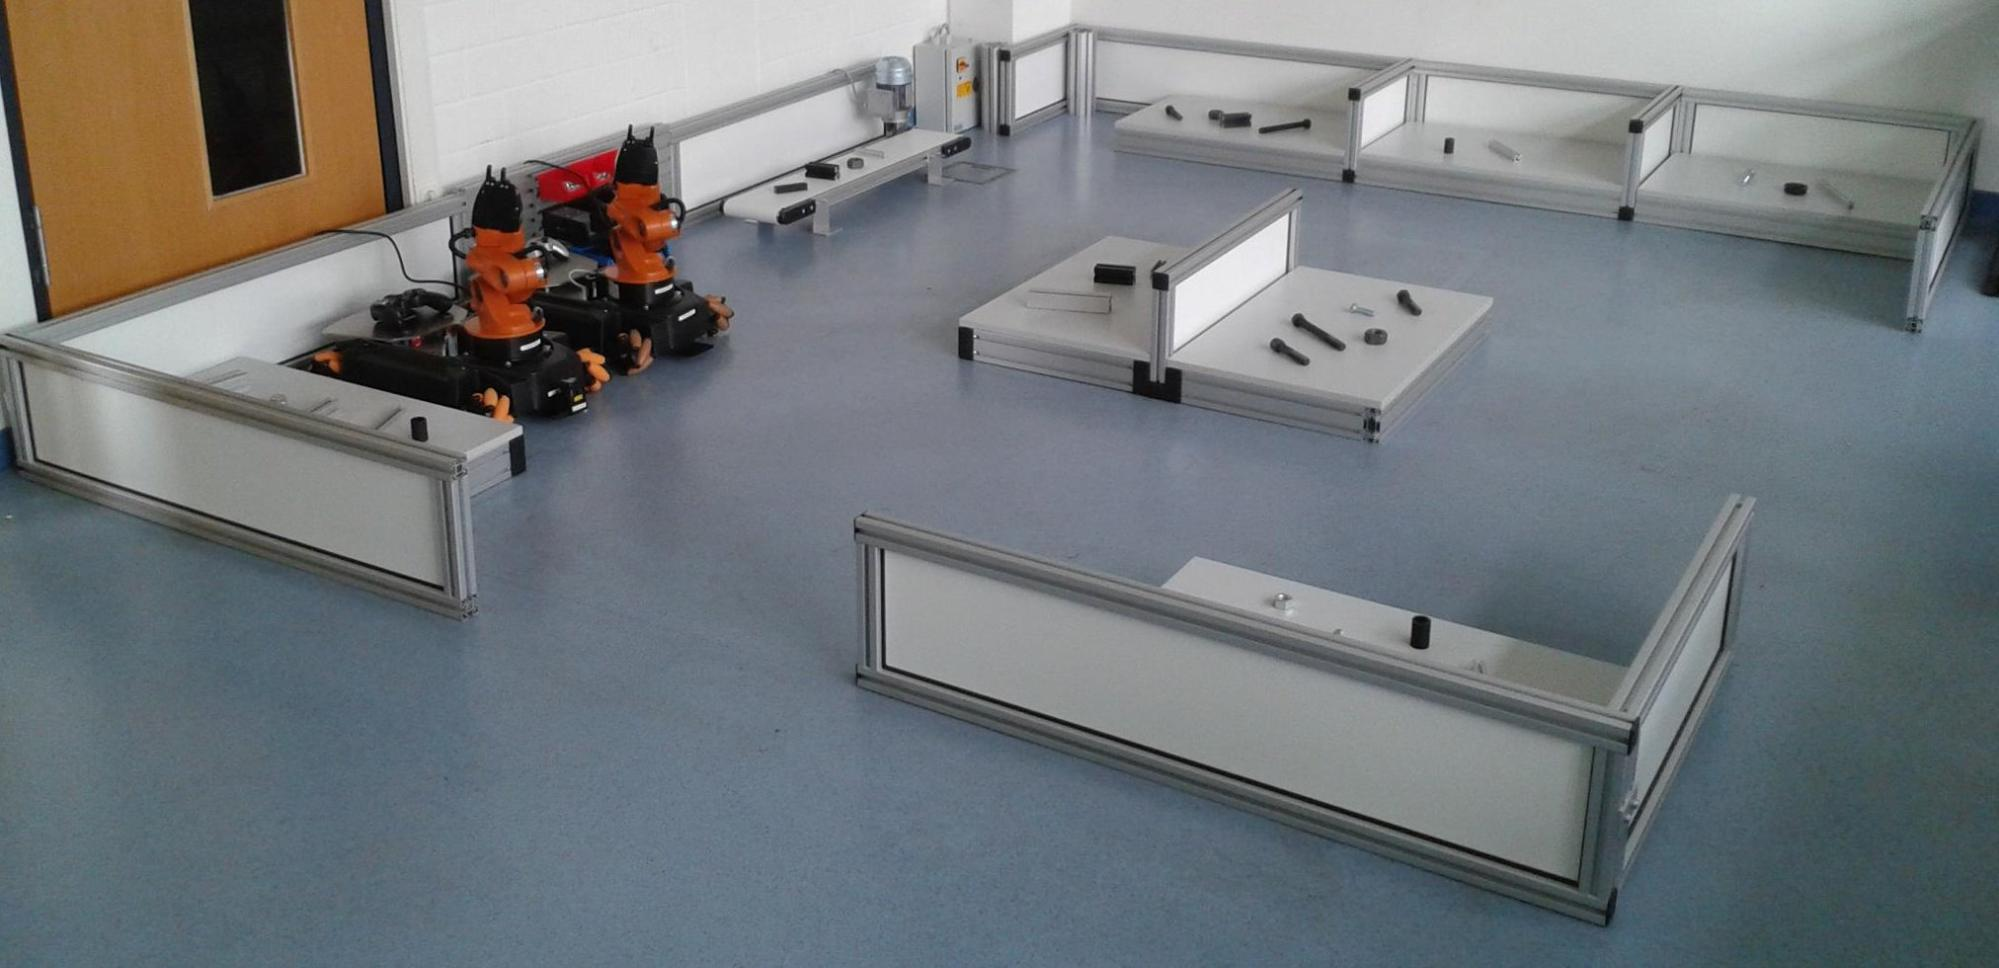
\includegraphics[width= \textwidth ]{../images/example_arena.jpg}
\caption{An exemplary setup for a RoboCup@Work environment}
\end{figure}

\subsection{Floor}
The floor is made of some firm material. Examples include floors made of concrete, screed, timber, plywood, chipboard, laminated boards, linoleum, PVC flooring, or carpet. Some examples are illustrated in Figure \ref{example_floors}. Floors may neither be made of loose material of any kind (gravel, sand, or any material which may damage the functioning of the robots’ wheels) nor may such material be used on top of the floor. Liquids of any kind are not allowed. The floor may have spots of unevenness of up to 1cm in any direction (clefts, rifts, ridges, etc.).

\begin{figure}
\begin{center}
\subfloat[]{
\includegraphics[width = 2cm]{../images/example_floor_1.jpg}}
\subfloat[]{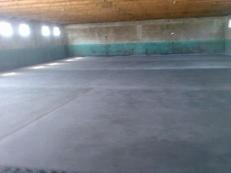
\includegraphics[width = 2cm]{../images/example_floor_2.jpg}} 
\subfloat[]{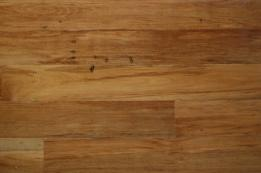
\includegraphics[width = 2cm]{../images/example_floor_3.jpg}} 
\subfloat[]{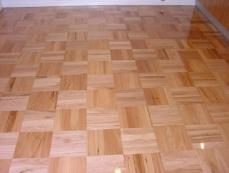
\includegraphics[width = 2cm]{../images/example_floor_4.jpg}}
\subfloat[]{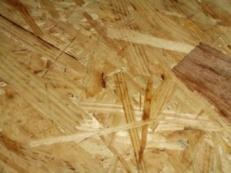
\includegraphics[width = 2cm]{../images/example_floor_5.jpg}}\\
\subfloat[]{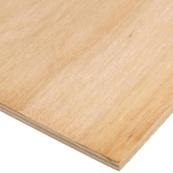
\includegraphics[width = 2cm]{../images/example_floor_6.jpg}} 
\subfloat[]{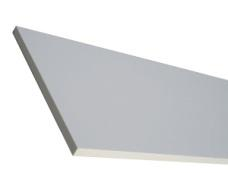
\includegraphics[width = 2cm]{../images/example_floor_7.jpg}} 
\subfloat[]{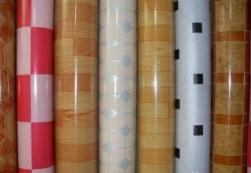
\includegraphics[width = 2cm]{../images/example_floor_8.jpg}} 
\subfloat[]{
\includegraphics[width = 2cm]{../images/example_floor_9.jpg}}
\subfloat[]{
\includegraphics[width = 2cm]{../images/example_floor_10.jpg}} 
\end{center}

\caption{Examples of floors that can be used for RoboCup@Work arenas.}
\label{example_floors}
\end{figure}

\subsection{Walls}
The competition arena is partly surrounded by walls. The height of the walls is no less than 20 cm and no more than 40 cm. One or more gates may be foreseen, where robots can enter or leave the arena. Gates may or may not be closable. The walls have a mostly uniform color.

\subsection{Service Areas}
Arenas contain one or more service areas, which have specific purposes for a particular test. Examples include loading and unloading areas, conveyor belts, rotators, storage areas, etc. Service areas may contain specific environment objects, such as racks, shelves, etc. 

\subsection{Racks}
Service areas, e.g. loading and unloading areas, may foresee the use of racks. Objects to be delivered or removed from racks have to be placed or picked up from the top. The height of the racks should be no less than 5 cm and no more than 40 cm. The color for the top surface of racks is white, unless a test specifies a different color. The top surface of the rack may be specially designed in order to serve specific purposes, e.g. holding objects. 

\subsection{Shelves}
Service areas may foresee the use of shelves and shelf units. Objects to be delivered or removed from shelves have to be placed or picked sideways. The height of the shelves should be no less than 5 cm and no more than 40 cm. The color of the shelf surface is white, unless a test specifies a different color. The shelf surface may be specially designed in order to serve specific purposes, e.g. holding objects. 

\subsection{Places}
An arena designed for a particular test may foresee the definition of a set of designated places, which are locations in the arena that can be referred to by a unique, symbolic identifier. These identifiers are used e.g. for task specification, possibly in conjunction with other information, such as an orientation. Places may be marked by markers of some sort. 

\subsection{Obstacles}
An arena defined for a particular test may foresee the use of obstacles. Obstacles may by passive (i.e. not able to relocate by themselves) or active (e.g. other robots). The size of obstacles should be no less than 10 cm x 10 cm x 5 cm; there is no upper bound on the size. The details about the dynamic objects are not known before the competition and will be chosen by the OC onsite. Examples for obstacles are trash bins, boxes, big aluminium profiles or even other robots.

\subsection{Floor Markers}
The arena used for a particular test may foresee the use of floor markers for designated places. The design of these floor markers are rectangular black-and-white images as used by the ARToolKit library:

http://www.hitl.washington.edu/artoolkit/

The black inner square of the markers is at least 8 cm x 8 cm large with an additional white border around of at least 12 cm side length. Figure \ref{fig:floor_marker} depicts some examples of these markers.

\begin{figure}
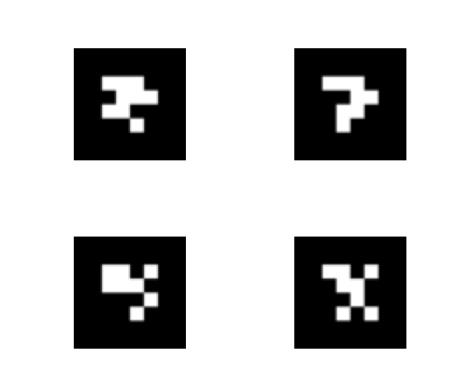
\includegraphics[width= 0.5\textwidth ]{../images/example_floor_marker.png}
\caption{Example of a floor marker.}
\label{fig:floor_marker}
\end{figure}


\subsection{Barrier Tape as Virtual Walls}
The arena may include virtual walls marked by either striped yellow and black or white and red barrier tape on the floor (see Figure \ref{fig:barrier_tape}). If any part of a robot passes over such a tape it is considered like a collision with a normal wall.

\begin{figure}
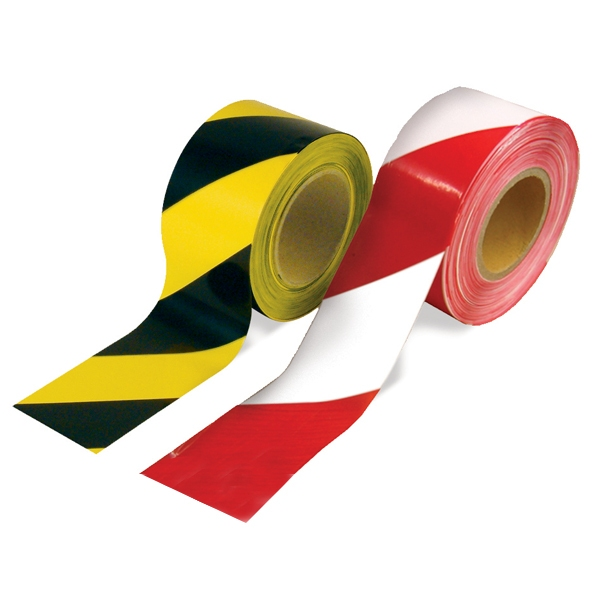
\includegraphics[width= 0.5\textwidth ]{../images/example_barrier_tape.jpg}
\caption{Example of Barrier Tape.}
\label{fig:barrier_tape}
\end{figure}

\subsection{Entrance and Exit}
If possible the Arena should have one entrance and one exit, which are equipped with Laser barriers. These barriers are used for timekeeping and will be used by the Referee Box. 

\subsection{Setup of the Arena}
The arena must be surrounded by either walls or barrier tape. The only exceptions are the Entrance and Exit. There must be a route to all places and markers relevant for a test which has a minimum width of 55 cm..

\section{Design of Manipulation Tasks}

\subsection{Manipulation Objects}
The manipulation objects in RoboCup@Work shall include a wide range of objects relevant in industrial applications of robotics and eventually cover any raw material, semi-finished parts, and finished parts and products as well as tools and possibly operating materials required for manufacturing processes. 
\par
The intention is to start with a simple set of objects of different shapes and colors and to widen the spectrum every year in at least one aspect. The initial set of objects includes basic and standard screws and nuts in various sizes and weight as shown in the following table:




\begin{table}[p]
\begin{tabular}{|c|c|c|c|}
\hline 
 & Symbolic Description & Weight (in g) & Details \\ 
\hline 
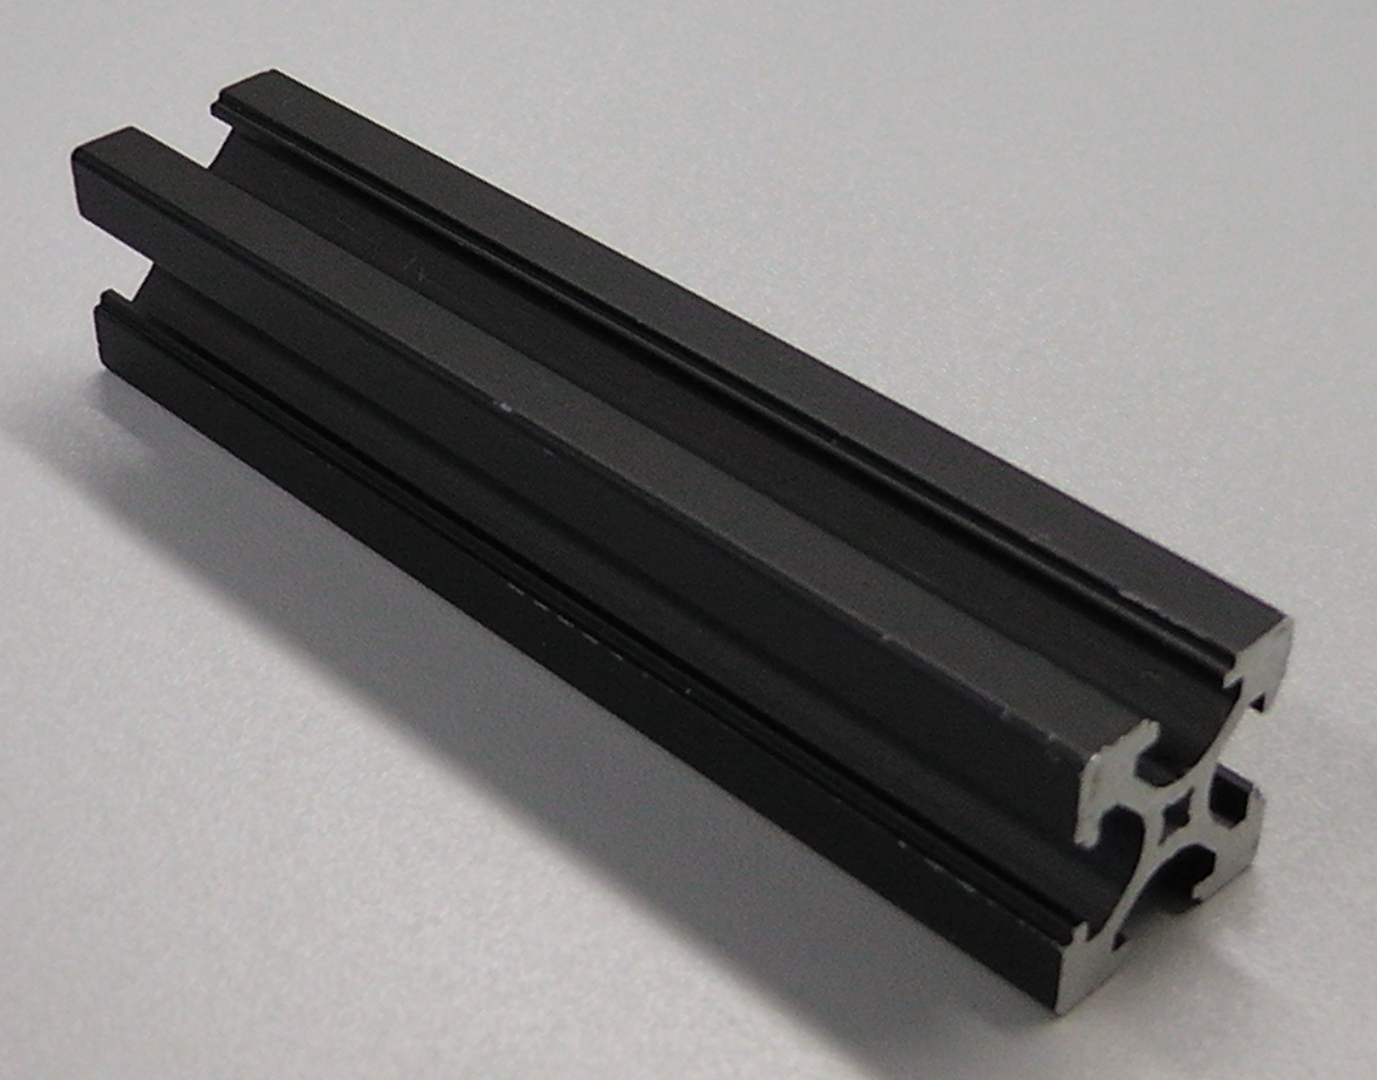
\includegraphics[width=3cm]{../images/F20_20_B.jpg} & F20\_20\_B & 49g & Height: 20mm \newline
 Width: 20mm \newline
 Length: 100mm \\ 
\hline 
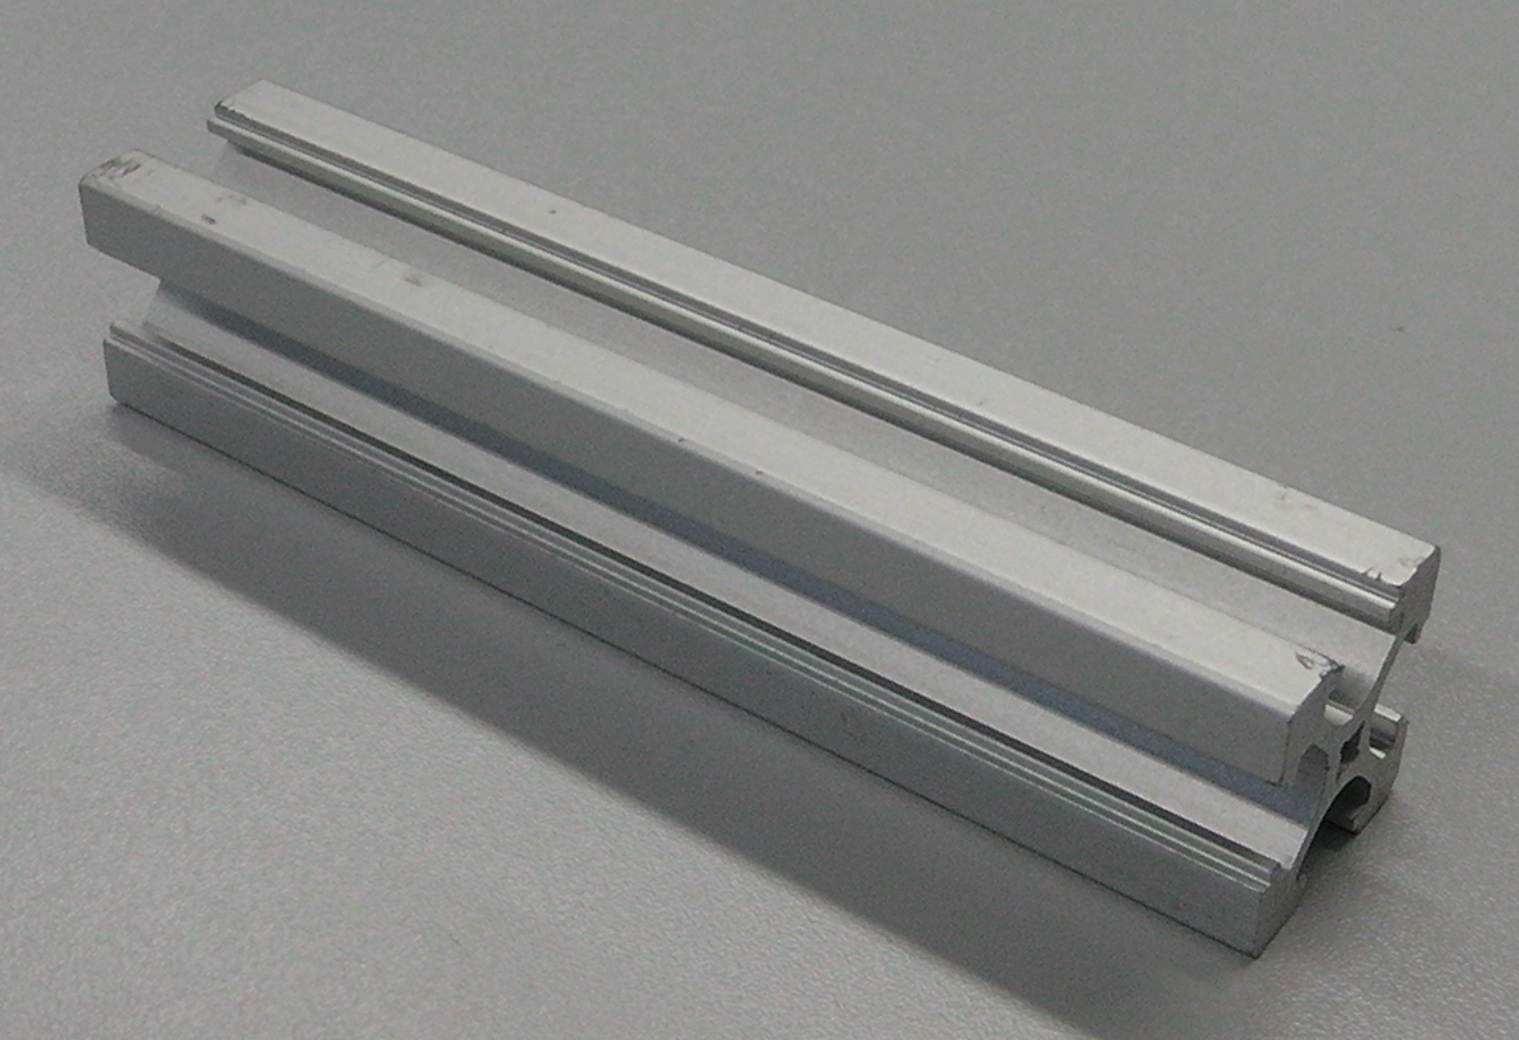
\includegraphics[width=3cm]{../images/F20_20_G.jpg} & F20\_20\_G & 49g & Height: 20mm \newline
Width: 20mm \newline
Length: 100mm \\ 
\hline 
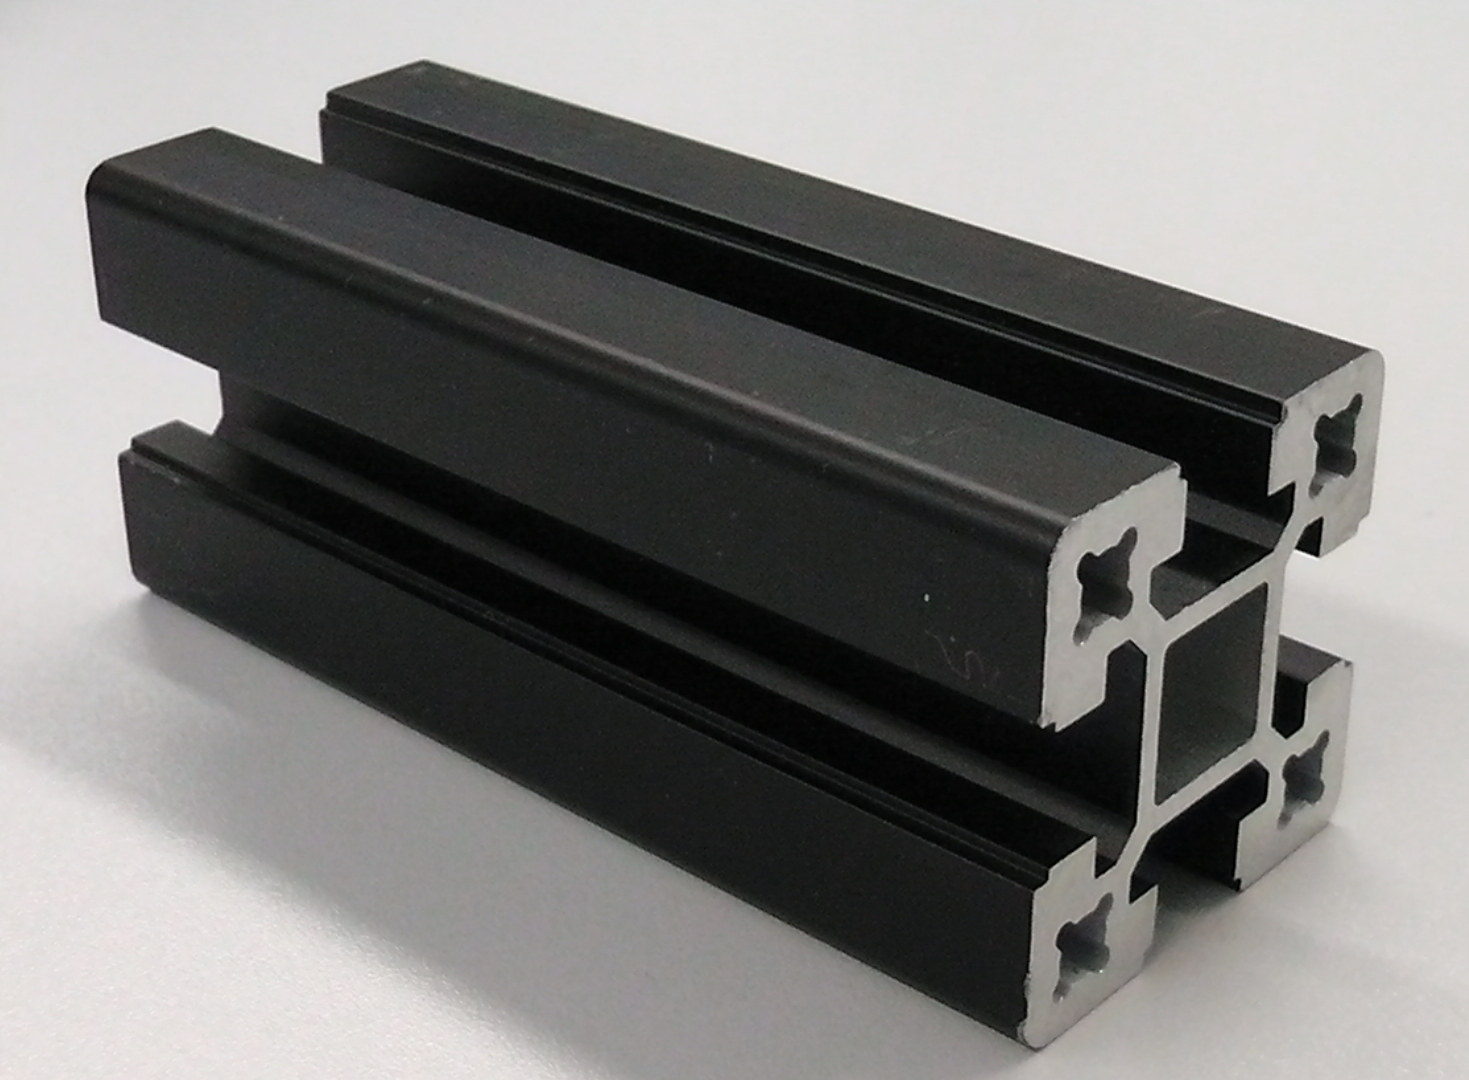
\includegraphics[width=3cm]{../images/S40_40_B.jpg} & S40\_40\_B & 186g & Height: 40mm \newline
Width: 40mm \newline
Length: 100mm \\ 
\hline 
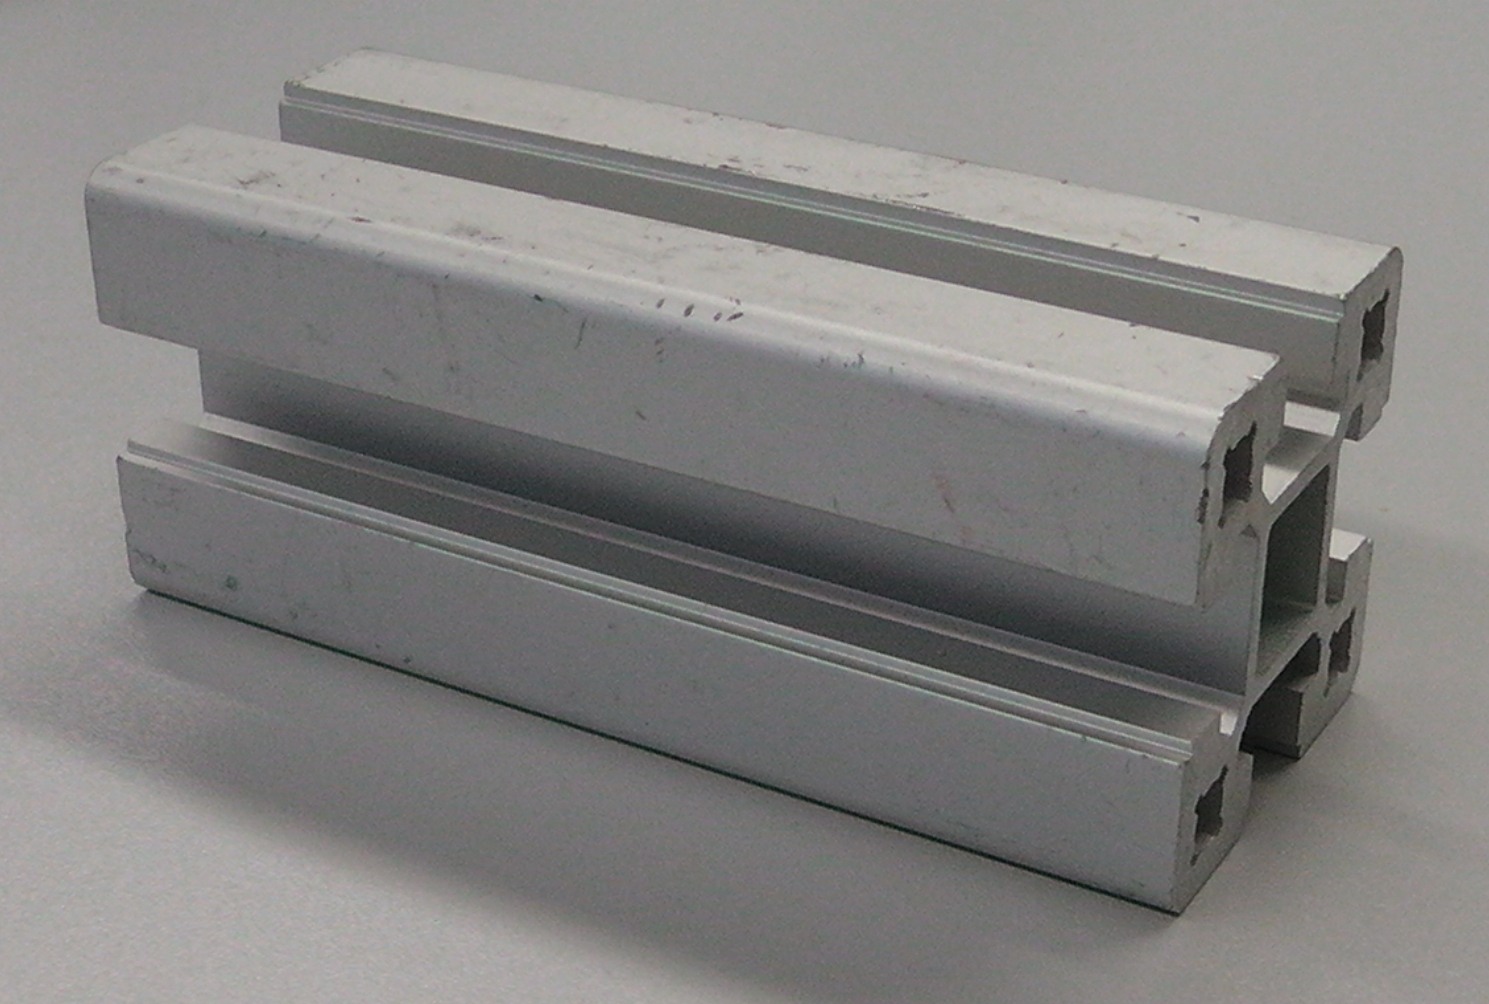
\includegraphics[width=3cm]{../images/S40_40_G.jpg} & S40\_40\_G & 186g & Height: 40mm \newline
Width: 40mm \newline
Length: 100mm \\ 
\hline 
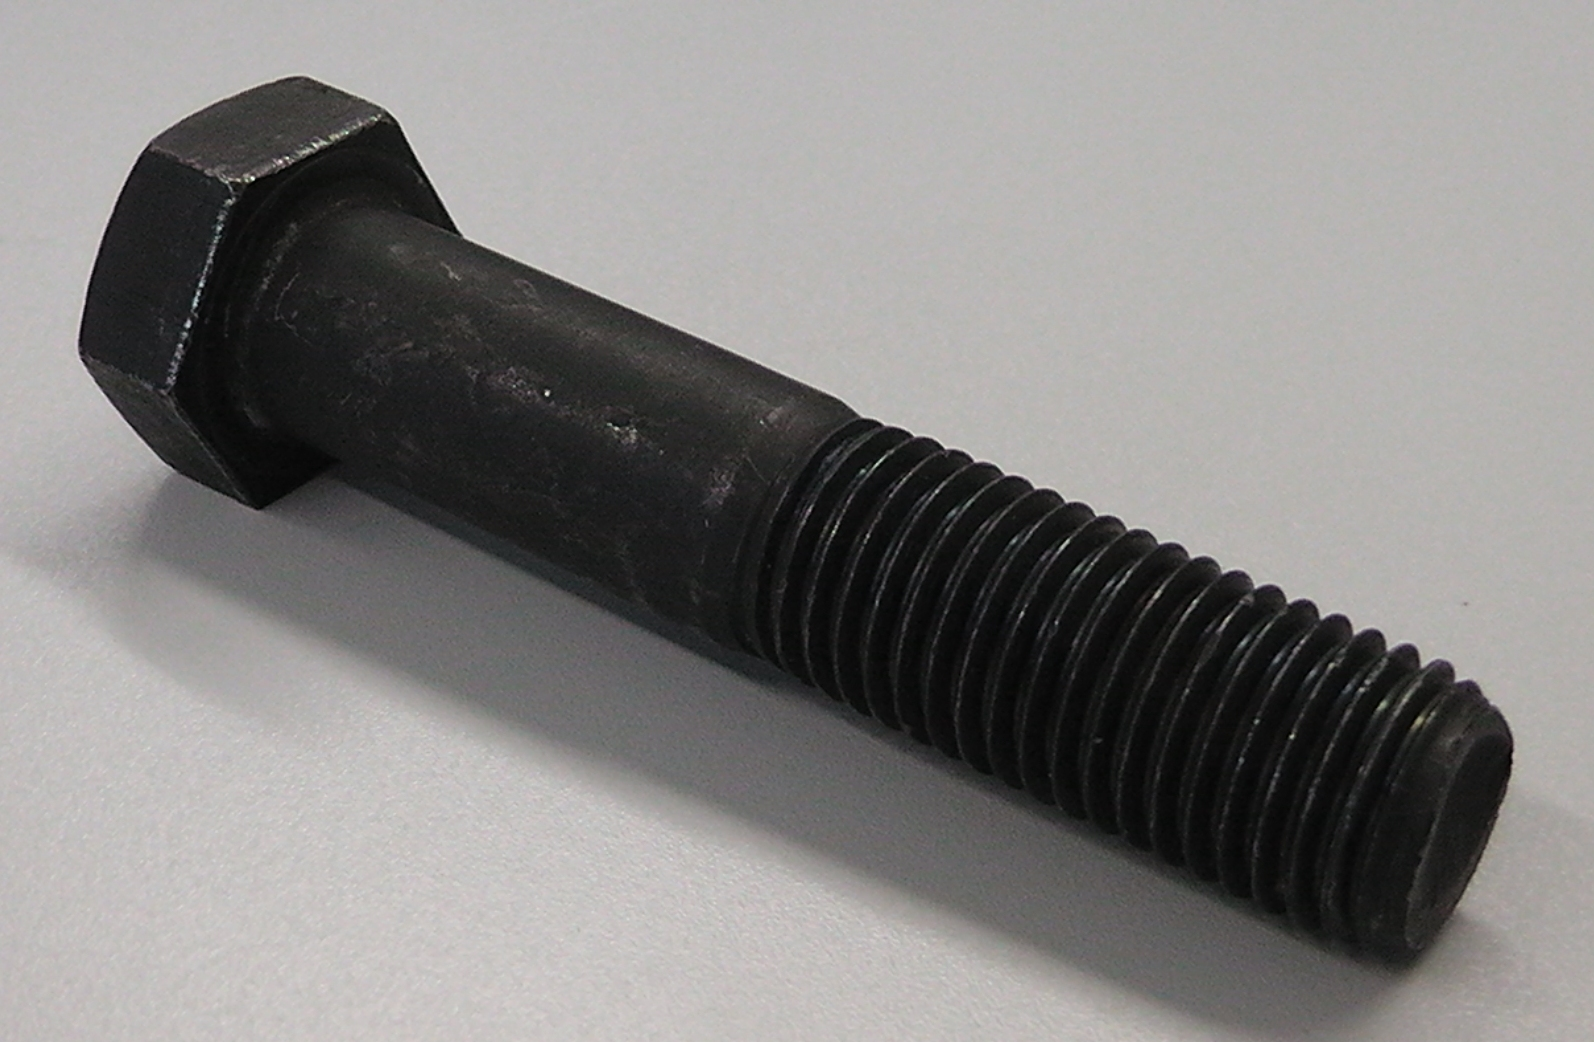
\includegraphics[width=3cm]{../images/M20_100.jpg} & M20\_100 & 296g & ISO 4014 \newline
M20 \newline
Length: 100mm \\ 
\hline 
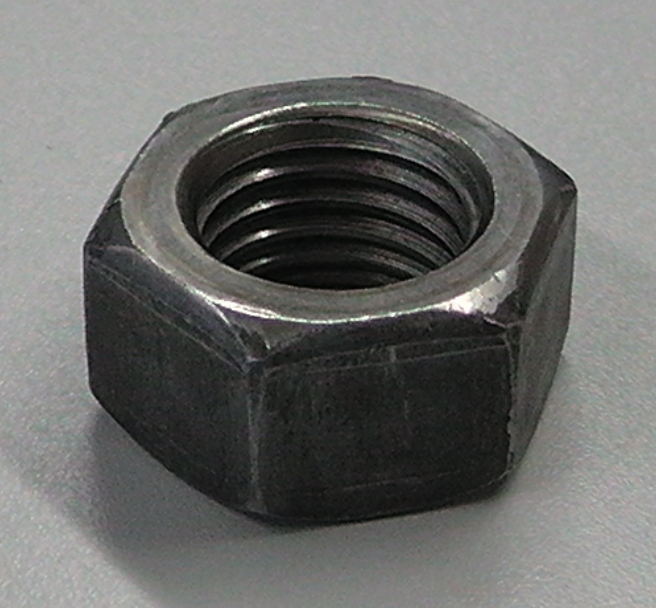
\includegraphics[width=3cm]{../images/M20.jpg} & M20 & 56g & ISO 4032 \newline M20 \\
\hline 
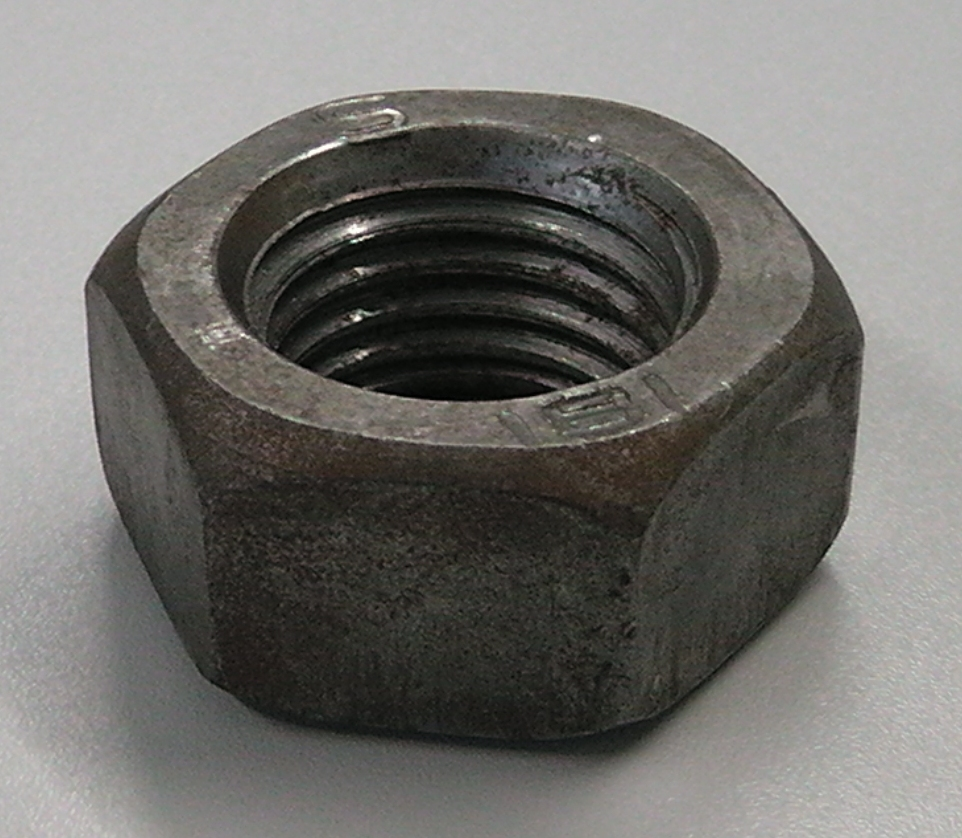
\includegraphics[width=3cm]{../images/M30.jpg} & M30 & 217g & ISO 4032 \newline M30 \\ 
\hline 
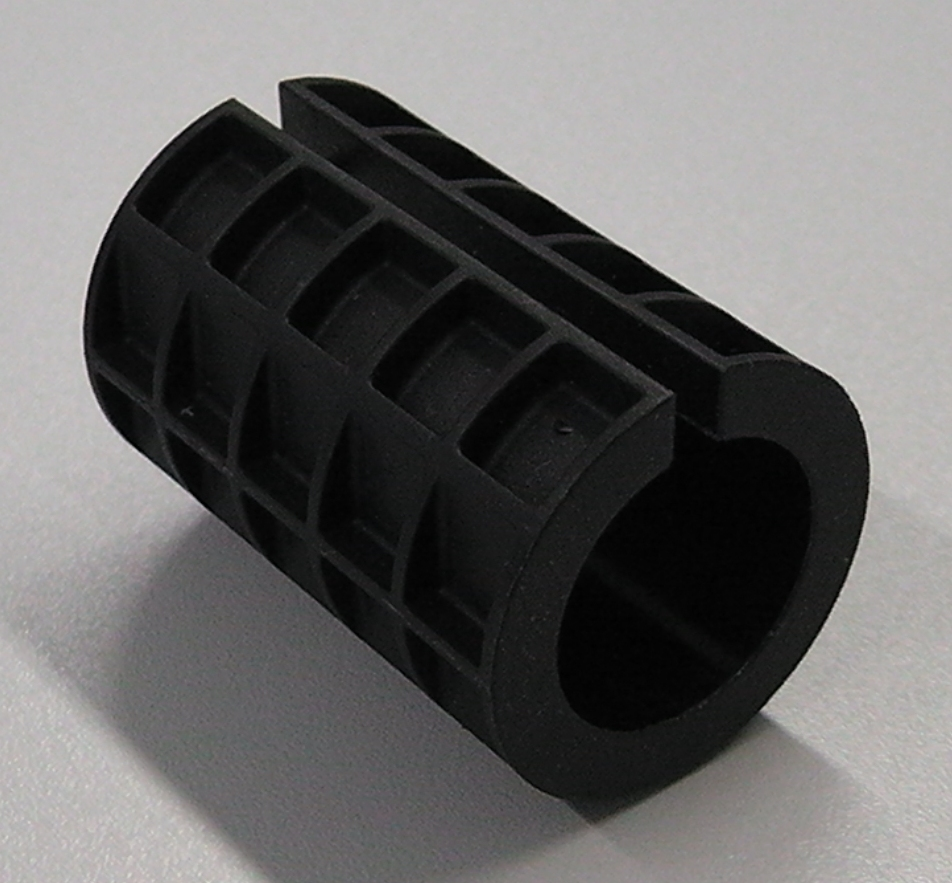
\includegraphics[width=3cm]{../images/R20.jpg} & R20 & 14g & Inner diameter: 20mm \newline
Outer diameter: 30mm
Length: 45mm \\ 
\hline 
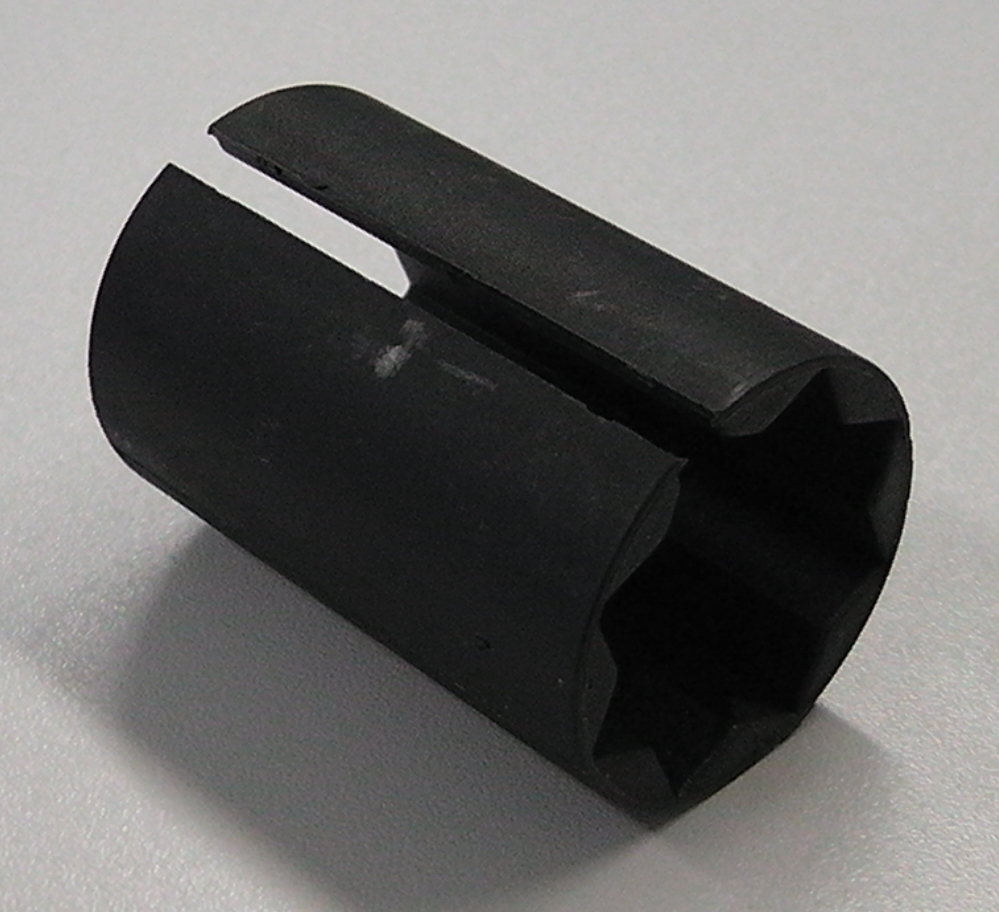
\includegraphics[width=3cm]{../images/V20.jpg} & V20 & 14g & Inner diameter: 20mm \newline
Outer diameter: 30mm \newline
Length: 45mm \\ 
\hline 
\label{tab:manipulation_objects}
\end{tabular} 

\caption{Examples of typical manipulation objects}

\end{table}

Objects of one kind can slightly vary e.g. considering surface. Teams can ask the Technical Committee for allowance to use objects brought by the team to a competition, provided they do not differ in a relevant way from the default objects.

\subsection{Manipulation Zone}

\subsection{Placement of objects}
For the placement of manipulation objects the following terms are used:

\begin{itemize}
\item position: point within 2D coordinate system of service area
\item rotation: rotation around vertical axis of service area
\item orientation: rotation around horizontal axes of service area, i.e. whether the object is standing upright or lying on its side.
\item pose: combination of position and rotation
\end{itemize}

\subsection{Grasping objects}
If not specified differently in a test, the following definition applies to decide if an object counts as grasped from a service area. 
\par
An object counts as grasped from a service area, when
the robot has lifted the object. It is not enough to shove it beyond the service areas edge.
the object was moved outside of the source service area. Outside means that the vertical projection of the object’s convex hull does not touch the service area anymore.
the robot shows the intention to move itself with the object away from the service area. By default this is assumed when the distance on the horizontal plane between every part of the robot and service area as well as between every part of the object and service area is more than 20 cm; or when the object has been placed on another service area. The referees may interpret the intention differently if agreed on before the run.
\par
The last point shall enable to let the robot pick up an object in order to analyse its type, e.g. by holding it close to a camera on the robot. 
\par
If the robot handles an object, but does not fulfil all points above, the object does not count as grasped, and neither points for grasping a required object, nor penalty points for grasping an unspecified object are given. Still, if the object drops to the ground or an uncontrolled collision occurs, the normal penalty points apply.

\subsection{Placing objects on service areas}
If not specified differently in a test, a manipulation object counts as placed on a target service area if any part of the object is touching the surface of the service area and the object is not moving at the end of the run.
\par
The position, rotation or orientation of the object on the service area can be chosen freely by the robot.

\section{Overall Scenario and Variation Points}
The following two figures illustrate the kind of arenas that can be built with the previously described components. Figure \ref{fig:example_map} shows an old arena configuration (from IROS 2012) as a topological map defining places and connections, while Figure \ref{fig:example_map_go13} shows an arena configuration (from German Open 2013) with only a few surrounding walls, more open space and a conveyor belt.

\begin{figure}
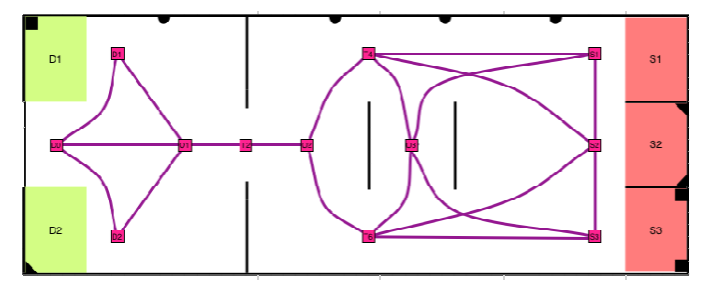
\includegraphics[width= \textwidth ]{../images/example_map.png}
\caption{Example of an arena with 5 service areas (D1, D2, S1, S2, S3). The purple squares define places.}
\label{fig:example_map}
\end{figure}

\begin{figure}
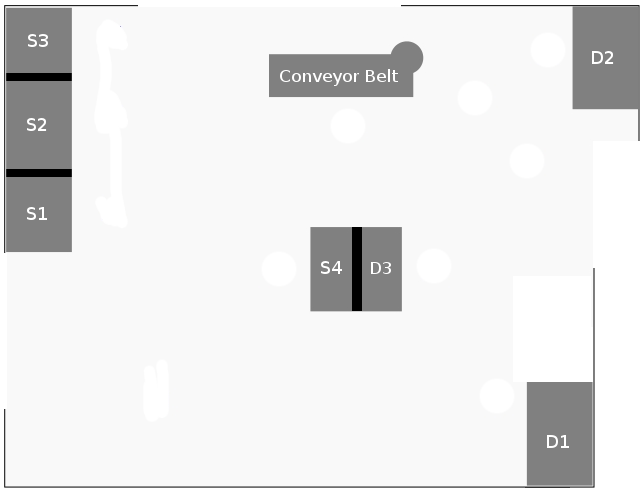
\includegraphics[width= \textwidth ]{../images/example_map_go13.png}
\caption{Illustration of the arena configuration used at the German Open 2013.}
\label{fig:example_map_go13}
\end{figure}

